% Copy the subsection and figure blocks into the supplementary manuscript.
% This minimal wrapper supports compilation in the document editor.
\documentclass[10pt,a4paper]{article}
\pdfminorversion=7
\usepackage[margin=22mm]{geometry}
\usepackage[T1]{fontenc}
\usepackage{lmodern}
\usepackage{amsmath,graphicx}
\begin{document}

\subsection*{Supplementary Method 9. \(N_{\mathrm{eff}}^{+}\) recovery simulations}

We simulated 100 paired trials using fully sampled pure-birth trees with a
crown age of 300~Ma. Speciation rates were $0.010$, $0.028$, and
$0.010~\mathrm{Myr}^{-1}$ during 300--180, 180--80, and 80--0~Ma,
respectively; extinction was zero. Trees were retained if they contained
120--250 tips and ten eligible contemporaneous branches during the
elevated-speciation interval. Selection did not use character states or
correlation outcomes. Each accepted tree was used in both scenarios.

Each dataset comprised ten anatomical units with 20 binary characters per
unit. In the Correlated scenario, each unit was assigned a focal branch.
Each character underwent a forced $0\to1$ change at a uniformly sampled
position within that branch's elevated-speciation segment, then evolved
on the remaining focal branch and its descendants under equal rates,
$q_{01}=q_{10}=10^{-4}~\mathrm{Myr}^{-1}$. States before the origin and outside
this subtree remained~0. In the Independent scenario,
characters evolved from root state~0 on all branches under homogeneous
equal rates, $q_{01}=q_{10}=0.003~\mathrm{Myr}^{-1}$.

Using only the tree and tip states, we fitted ER models in \texttt{ontophylo}
with three optimization restarts and the \texttt{maddfitz} root treatment,
then generated 100 conditional stochastic maps per variable character.
Constant characters were excluded without redrawing, leaving 198--200
variable characters per Correlated trial and 200 per Independent trial.
Within each map, unit-specific branch rates were the summed mapped changes
divided by branch duration. Rates strictly above the unit's 95th percentile
across branches were classified as accelerated; constant rate vectors were
left unclassified.

At each 1-Myr midpoint, we calculated
\[
N_{\mathrm{eff}}^{+}=f\exp\!\left(-\sum_k p_k\log p_k\right),
\]
where $f$ is the fraction of contemporaneous lineages with at least one
accelerated unit, and $p_k$ is the frequency of nonzero joint acceleration
pattern $k$ among those lineages. The metric was zero when none were
accelerated. We calculated it separately within each map before averaging
across maps. Figure~\ref{fig:neff-publication-trajectories} shows all trial
means and their mean across trials, alongside the known speciation schedule
and the prespecified example tree (trial 001).

For each trial, we averaged reconstructed $N_{\mathrm{eff}}^{+}$ and known
diversification ($\lambda-\mu=\lambda$) within 15 matched, non-overlapping
20-Myr bins and calculated a two-sided Pearson correlation.
Figure~\ref{fig:neff-publication-associations} shows the coefficients,
$p$-values, and fractions of trials with $p<0.05$. These nominal tests do not
adjust for temporal autocorrelation; the Independent scenario evaluates
false-association frequency under the specified simulation design.

\begin{figure}[p]
\centering
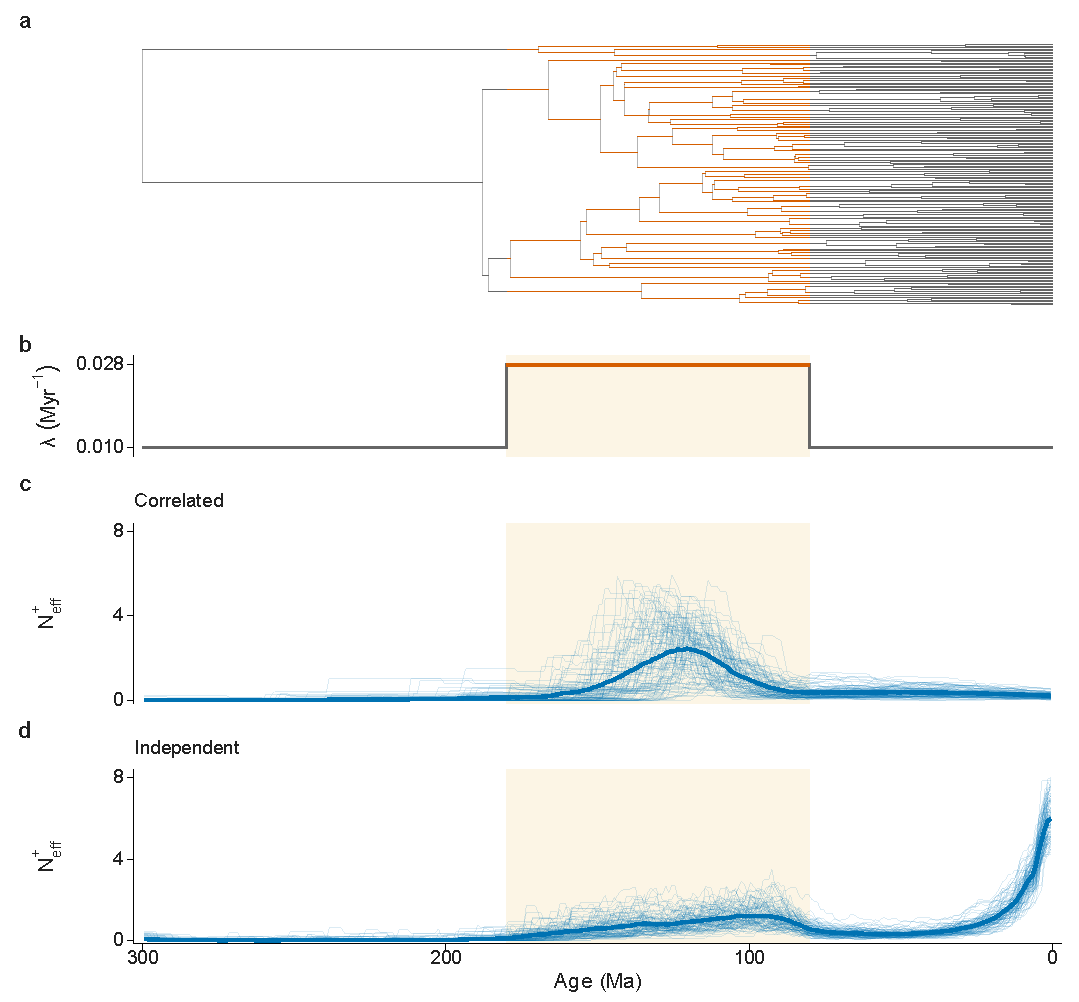
\includegraphics[width=\textwidth]{figures/figure-1-neff-and-diversification.pdf}
\caption{\textbf{Reconstructed phenomic diversity in the Correlated and
Independent scenarios.} (a) Example simulated tree (trial 001), with branch
segments coloured by the generating speciation rate: grey,
$\lambda=0.010~\mathrm{Myr}^{-1}$; orange,
$\lambda=0.028~\mathrm{Myr}^{-1}$. (b) Speciation schedule shared by all
trials. Extinction was zero, so $\lambda$ also represents net diversification.
(c,d) Reconstructed $N_{\mathrm{eff}}^{+}$ trajectories for 100 trials per
scenario, with trees paired between scenarios. Thin lines show individual
trial means across 100 conditional stochastic maps per variable character;
thick lines show means across trials. Both diversity panels use the same
vertical scale. Shading marks the elevated-speciation interval (180--80~Ma).
The Correlated scenario was designed to generate a positive association by
concentrating character origins on contemporaneous branches within this
interval, followed by slow character evolution. The Independent scenario
used homogeneous equal-rates character evolution independent of the
diversification regime. Diversity was reconstructed from tip observations
using the strict acceleration cutoff.}
\label{fig:neff-publication-trajectories}
\end{figure}

\begin{figure}[p]
\centering
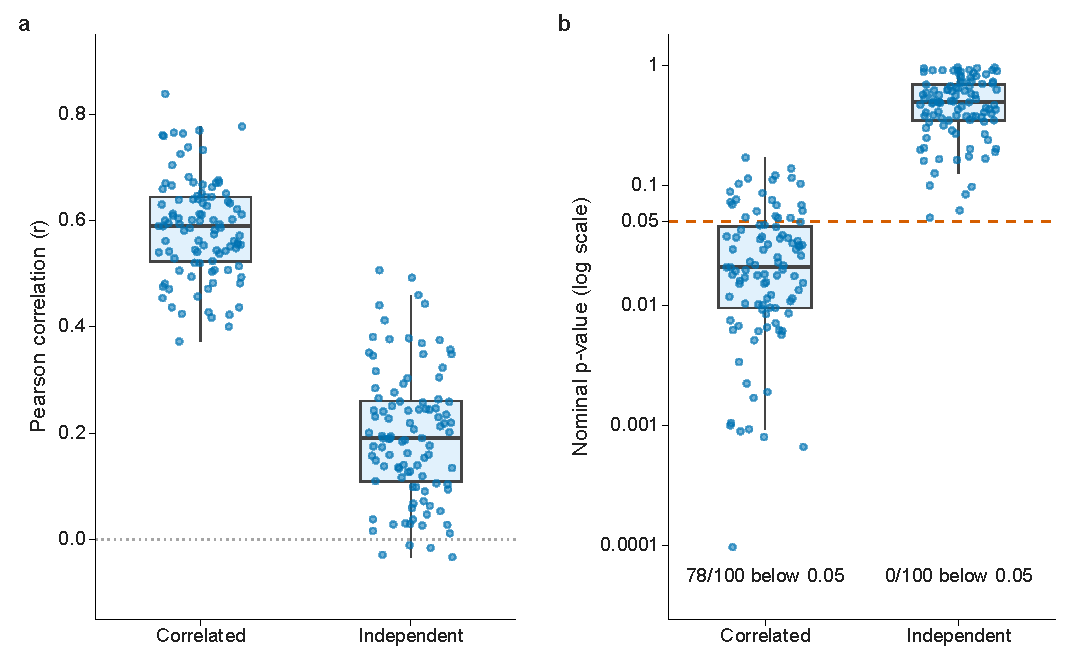
\includegraphics[width=\textwidth]{figures/figure-2-correlations-and-p-values.pdf}
\caption{\textbf{Correlations between reconstructed phenomic diversity and
known diversification.} (a) Pearson correlation coefficients between
reconstructed $N_{\mathrm{eff}}^{+}$ and generating diversification.
(b) Corresponding nominal two-sided $p$-values on a logarithmic axis.
Correlations were calculated across 15 matched, non-overlapping 20-Myr bins
for the scenarios in Figure~\ref{fig:neff-publication-trajectories}.
Each point represents one trial ($n=100$ per scenario); horizontal jitter
separates overlapping points. Boxes show interquartile ranges, central bars
show medians, and whiskers extend to the most extreme observations within
1.5 interquartile ranges of the box edges. Boxplot summaries are calculated
on the displayed scales. The grey dotted line marks $r=0$; the orange dashed
line marks $p=0.05$. Nominal $p<0.05$ occurred in 78 of 100 Correlated trials
and none of the 100 Independent trials. Tests use the strict acceleration
cutoff and do not adjust for temporal autocorrelation.}
\label{fig:neff-publication-associations}
\end{figure}
\end{document}
